\documentclass[11pt]{article}
\usepackage[margin=1.0in]{geometry}

% Required packages
\usepackage{amsmath,amsfonts,amsthm,amssymb} % Mathematical typesetting and symbols
\usepackage{bigstrut} % Row spacing
\usepackage{enumerate} % Custom enumerate labels
\usepackage{esint} % Alternate double integral symbols
\usepackage{fancyhdr} % Headers and footers
\usepackage{graphicx} % Figure inclusion
\usepackage{hyperref} % Hyperlinks for citations, references, and URLs
\usepackage{placeins} % Float barriers
\usepackage{slashbox} % Slash in a table cell
\usepackage{subcaption} % Captions for subfigures
\usepackage{titlesec} % Custom section labels
\usepackage{wrapfig} % Wrapping text around figures
\usepackage{xcolor} % Text color

% Label Sections as Parts
\titleformat{\section}{\normalfont\Large\bfseries}{Part \thesection:}{0.5em}{}

% Define license image
\newcommand{\licenseimage}{figures/by-sa.png}

% Footer for first page
\pagestyle{plain}
\renewcommand{\headrulewidth}{0pt}
\fancyhead{}
\fancyfoot{}
\cfoot{\includegraphics[width=0.75in]{\licenseimage} \\ \footnotesize This work by the \href{https://floridapoly.edu/academic-departments/applied-mathematics.php}{Department of Applied Mathematics at Florida Polytechnic University} is licensed under a \href{https://creativecommons.org/licenses/by-sa/4.0/}{Creative Commons Attribution-ShareAlike 4.0 International License}.}


%==============================================================================

\begin{document}

\noindent \makebox[\textwidth]{\textbf{\LARGE Introduction to Rates of Change}}

\quad

%% Update cover image
\begin{figure}[h]
	\centering
	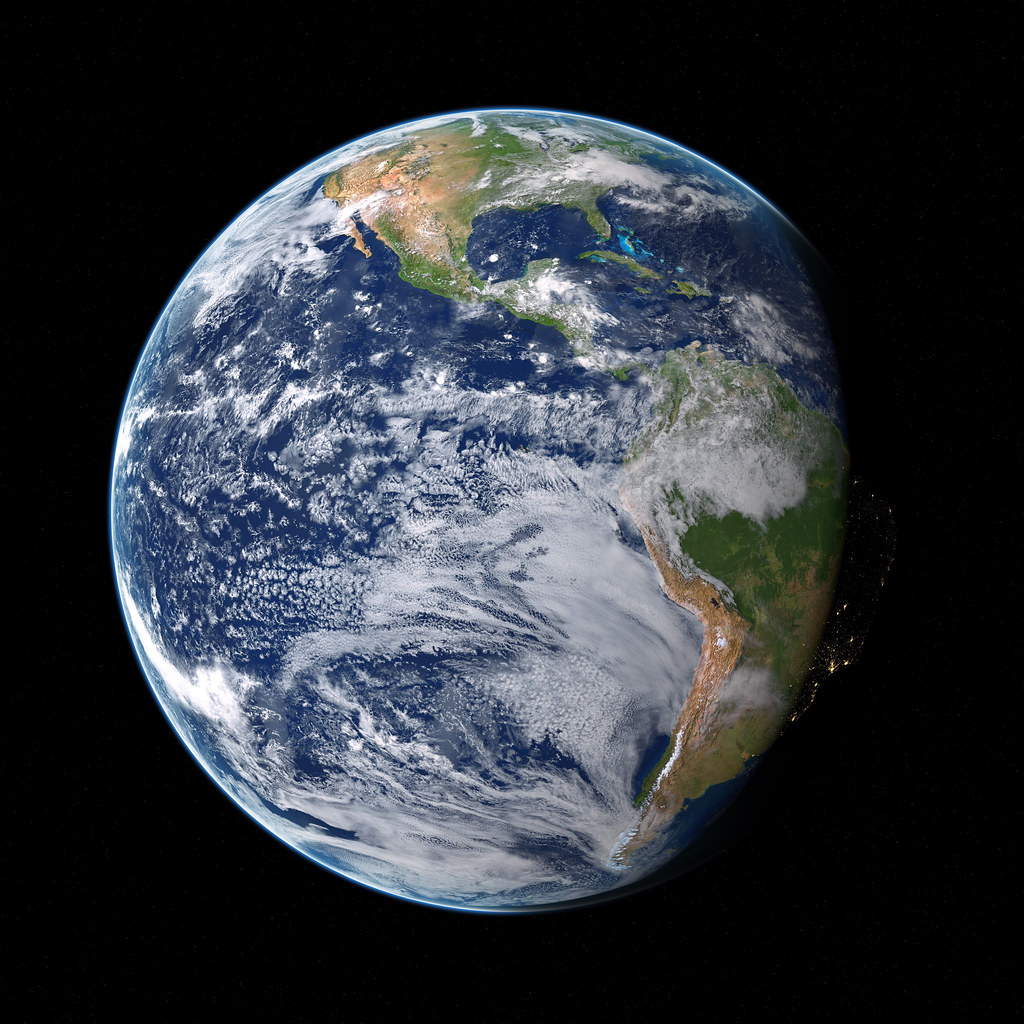
\includegraphics[width=0.45\textwidth]{figures/earth.jpg}
\end{figure}

%==============================================================================
\section*{Introduction}

\thispagestyle{fancy} % Add footer to first page only

\textcolor{red}{Introductory paragraphs}

%%%
\subsection*{Learning Objectives}

After completing this project, you should be able to:
\begin{itemize}
	\item \textcolor{red}{List of learning objectives}
\end{itemize}

% (Overall: Start with a very small data series and/or function, simple enough for the student to work with by hand, then move up to a very large data series.)
% In introducing the relationship between slopes and rates of change, ask the student why converting a numerical question into a geometric one might be useful. There are lots of possible answers, including the fact that it makes things easier to visualize and understand, and that it allows us to use all of the geometric things we know from precalculus (the idea of converting one kind of mathematical question into another is very common and useful since it allows us to reuse previous work to answer new questions).
% Start with a position function, and have the student compute some average velocities between different points.
% Then do the same thing, this time with a table of position values that the student generates from the given function.
% Introduce the idea of instantaneous velocity, and how it relates to slope.
% Estimate instantaneous velocity at a point, then repeat for all points to estimate the velocity function.
	% Answer some questions about how the two relate to each other geometrically.
% Focus on one point, and estimate the instantaneous velocity there using different step sizes. Note that they seem to settle down as the step size approaches zero.
% Plot the average velocity as a function of the step size. Note the #DIV/0! error when the step size is exactly zero, and the corresponding hole in the graph, but also note that everything seems well-behaved around that point, and motivate the idea of using limits to find what point "should" go there.

%==============================================================================
\section{\textcolor{red}{Section Title}}
\label{sec:sectiontitle}

\textcolor{red}{Section description}

%%%
\subsection*{Activity}

\textcolor{red}{Activity introduction}

\begin{enumerate}[\bf {\thesection}a.]
	\item \textcolor{red}{Parts of activity}
\end{enumerate}

\end{document}
